\documentclass[border=8pt]{standalone}
\usepackage{tikz}
\usepackage{amsmath,amssymb}
\usetikzlibrary{arrows.meta,positioning,decorations.pathmorphing,shapes.geometric,calc,fit}
\usepackage{xcolor}
\definecolor{Navy}{RGB}{27,73,101}
\definecolor{Rust}{RGB}{193,102,107}
\definecolor{Teal}{RGB}{77,144,142}
\definecolor{Gold}{RGB}{224,159,62}
\definecolor{Violet}{RGB}{110,80,170}

\begin{document}
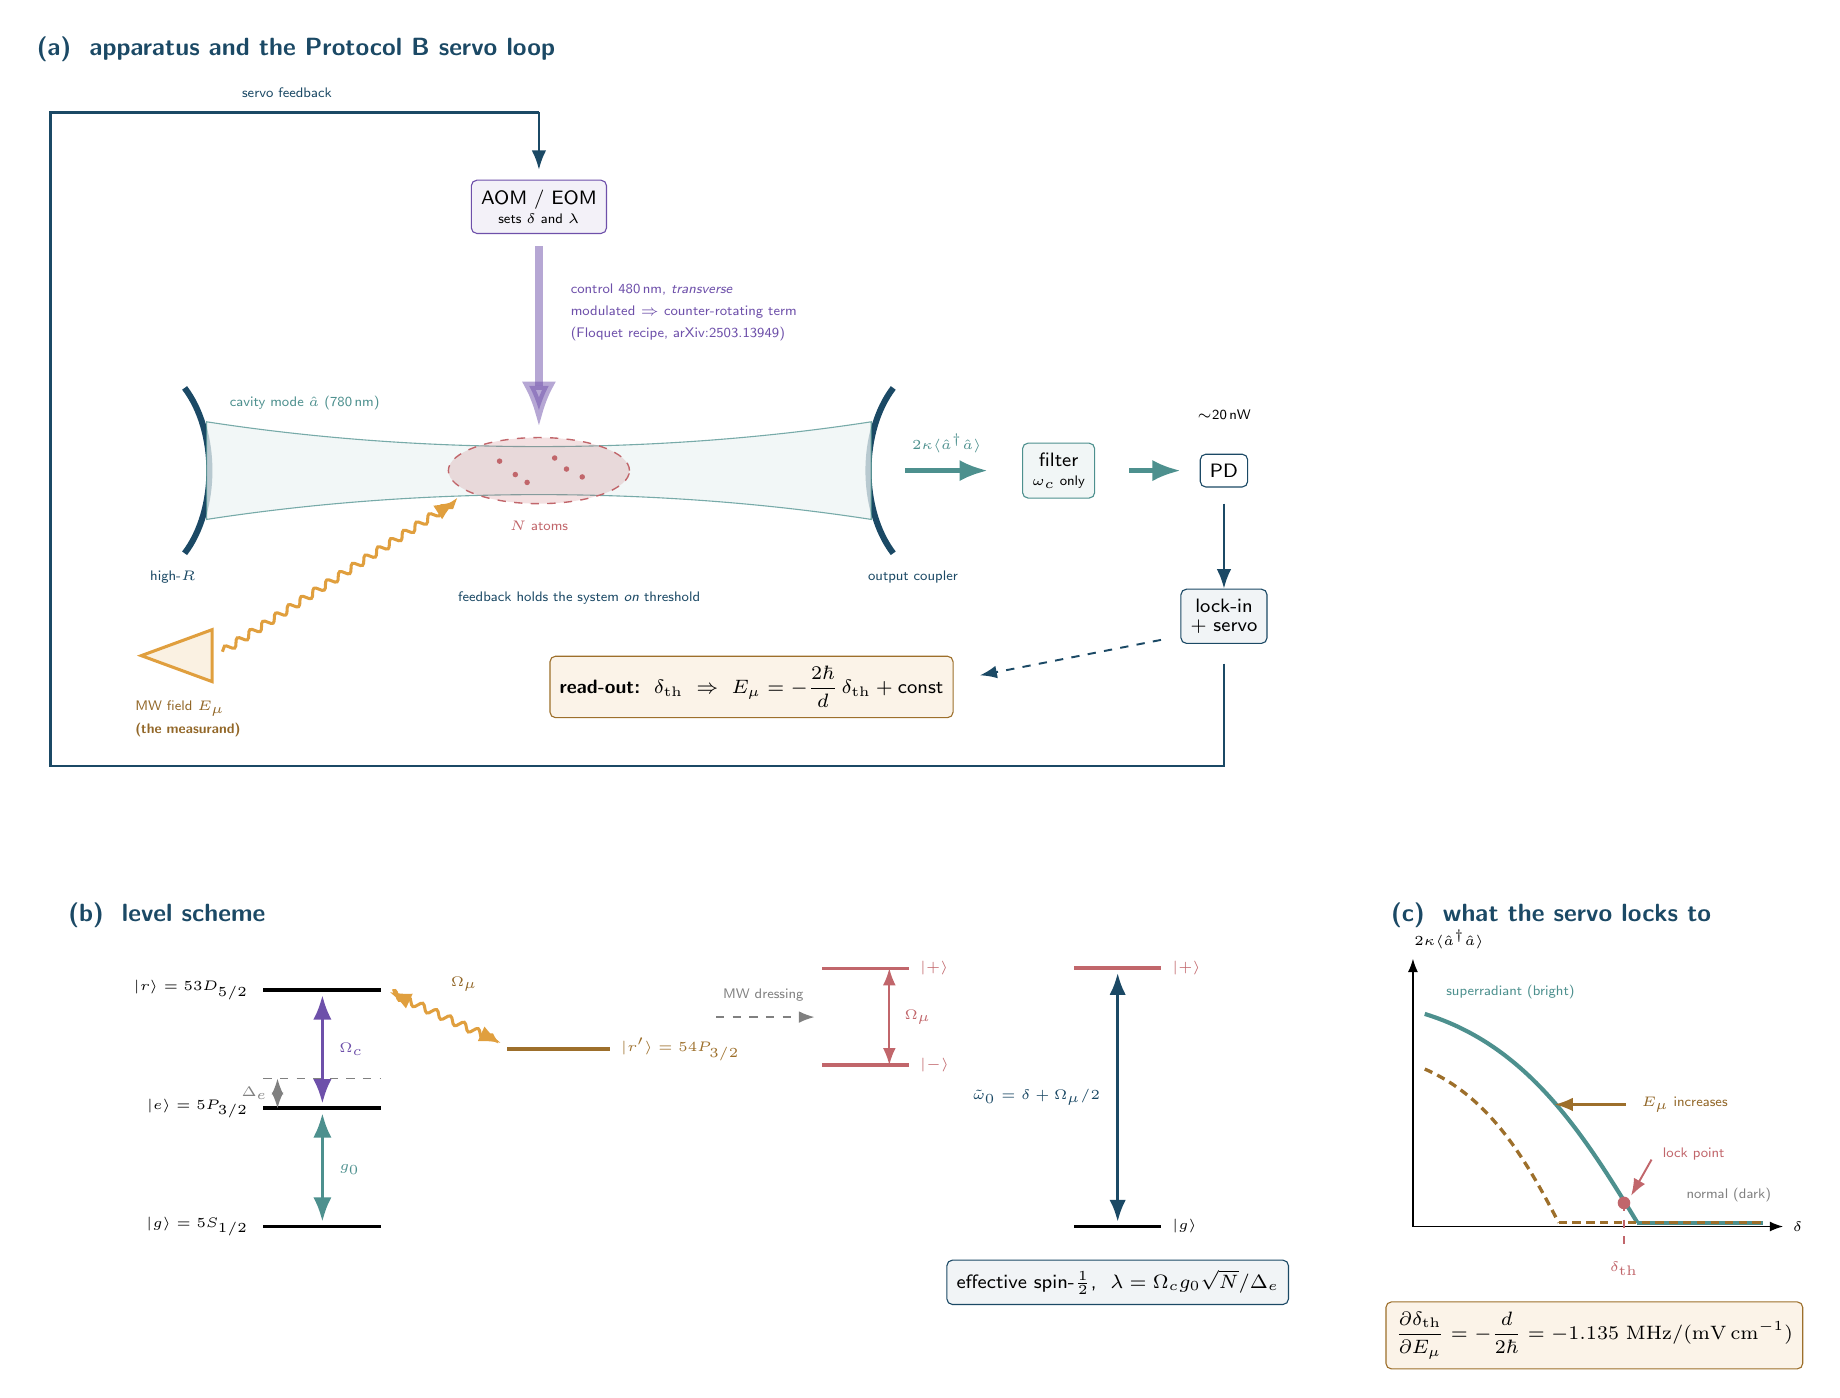
\begin{tikzpicture}[
  >=Latex, font=\sffamily,
  hdr/.style={font=\sffamily\small\bfseries, Navy},
  lbl/.style={font=\sffamily\scriptsize},
  tin/.style={font=\sffamily\tiny},
  box/.style={draw=Navy, fill=white, rounded corners=2pt, inner sep=3.5pt,
              font=\sffamily\scriptsize, align=center},
  mw/.style={decorate, decoration={snake, amplitude=1.3pt, segment length=5.5pt},
             Gold, line width=1.1pt},
  beam/.style={Violet, line width=3pt, opacity=0.5},
  loop/.style={Navy, line width=0.9pt},
]

%======================= (a) APPARATUS =======================
\node[hdr, anchor=west] at (-2.0,5.35) {(a)\ \ apparatus and the Protocol B servo loop};

% ---- feedback loop routed clear of the optics ----
\draw[loop] (13.2,-2.45) -- (13.2,-3.75) -- (-1.7,-3.75) -- (-1.7,4.55) -- (4.5,4.55);
\draw[loop,->] (4.5,4.55) -- (4.5,3.82);
\node[tin, Navy, anchor=south] at (1.3,4.62) {servo feedback};

% ---- cavity ----
\draw[line width=2.2pt, Navy] (0,-1.05) .. controls (0.42,-0.5) and (0.42,0.5) .. (0,1.05);
\draw[line width=2.2pt, Navy] (9,-1.05) .. controls (8.58,-0.5) and (8.58,0.5) .. (9,1.05);
\node[tin, Navy] at (-0.15,-1.35) {high-$R$};
\node[tin, Navy] at (9.25,-1.35) {output coupler};

\draw[Teal, fill=Teal!10, opacity=0.75, line width=0.4pt]
  (0.28,0.62) .. controls (3,0.20) and (6,0.20) .. (8.72,0.62)
  -- (8.72,-0.62) .. controls (6,-0.20) and (3,-0.20) .. (0.28,-0.62) -- cycle;
\node[tin, Teal, anchor=west] at (0.45,0.86) {cavity mode $\hat a$ (780\,nm)};

% ---- atoms ----
\fill[Rust, opacity=0.20] (4.5,0) ellipse (1.15 and 0.42);
\draw[Rust, dashed, line width=0.5pt] (4.5,0) ellipse (1.15 and 0.42);
\foreach \x/\y in {4.0/0.12, 4.35/-0.15, 4.7/0.16, 5.05/-0.08, 4.2/-0.05, 4.85/0.02}
  {\fill[Rust] (\x,\y) circle (0.035);}
\node[tin, Rust, anchor=north] at (4.5,-0.52) {$N$ atoms};

% ---- transverse control beam ----
\node[box, fill=Violet!8, draw=Violet] (aom) at (4.5,3.35) {AOM / EOM\\[-1pt]{\tiny sets $\delta$ and $\lambda$}};
\draw[beam, ->] (4.5,2.85) -- (4.5,0.55);
\node[tin, Violet, anchor=west] at (4.78,2.30) {control 480\,nm, \emph{transverse}};
\node[tin, Violet, anchor=west] at (4.78,2.02) {modulated $\Rightarrow$ counter-rotating term};
\node[tin, Violet, anchor=west] at (4.78,1.74) {(Floquet recipe, arXiv:2503.13949)};

% ---- microwave (the measurand) ----
\draw[Gold, line width=1.1pt, fill=Gold!15]
  (-0.55,-2.35) -- (0.35,-2.02) -- (0.35,-2.68) -- cycle;
\draw[mw, ->] (0.48,-2.30) -- (3.45,-0.38);
\node[tin, Gold!65!black, anchor=north west] at (-0.75,-2.80) {MW field $E_\mu$};
\node[tin, Gold!65!black, anchor=north west] at (-0.75,-3.08) {\textbf{(the measurand)}};

% ---- detection ----
\draw[Teal, line width=1.6pt, ->] (9.15,0) -- (10.2,0);
\node[box, fill=Teal!8, draw=Teal] (filt) at (11.1,0) {filter\\[-1pt]{\tiny $\omega_c$ only}};
\draw[Teal, line width=1.6pt, ->] (12.0,0) -- (12.65,0);
\node[box] (pd) at (13.2,0) {PD};
\node[tin, Teal, anchor=south] at (9.68,0.10) {$2\kappa\langle\hat a^\dagger\hat a\rangle$};
\node[tin, anchor=south] at (13.2,0.52) {$\sim$20\,nW};

\node[box, fill=Navy!6] (servo) at (13.2,-1.85) {lock-in\\[-1pt]+ servo};
\draw[loop,->] (13.2,-0.42) -- (servo);

\node[box, fill=Gold!12, draw=Gold!70!black, anchor=north] (out) at (7.2,-2.35)
   {\textbf{read-out:}\ \ $\delta_{\rm th}\ \Rightarrow\ E_\mu=-\dfrac{2\hbar}{d}\,\delta_{\rm th}+\text{const}$};
\draw[Navy, dashed, line width=0.7pt, ->] (12.4,-2.15) -- (10.1,-2.60);
\node[tin, Navy, anchor=west] at (3.35,-1.62) {feedback holds the system \emph{on} threshold};

%======================= (b) LEVELS =======================
\begin{scope}[shift={(-0.6,-9.6)}]
\node[hdr, anchor=west] at (-1.0,3.95) {(b)\ \ level scheme};
% bare ladder, labels on the LEFT so the right side is free
\draw[line width=1.4pt] (1.6,0)   -- (3.1,0)   node[left=1.55cm,tin] {$|g\rangle=5S_{1/2}$};
\draw[line width=1.4pt] (1.6,1.5) -- (3.1,1.5) node[left=1.55cm,tin] {$|e\rangle=5P_{3/2}$};
\draw[line width=1.4pt] (1.6,3.0) -- (3.1,3.0) node[left=1.55cm,tin] {$|r\rangle=53D_{5/2}$};
\draw[dashed, gray, line width=0.5pt] (1.6,1.88) -- (3.1,1.88);
\draw[<->, gray, line width=0.6pt] (1.78,1.5) -- (1.78,1.88) node[midway,left,tin] {$\Delta_e$};
\draw[Teal, line width=1.3pt, <->] (2.35,0.06) -- (2.35,1.44);
\node[tin, Teal, anchor=west] at (2.44,0.72) {$g_0$};
\draw[Violet, line width=1.3pt, <->] (2.35,1.56) -- (2.35,2.94);
\node[tin, Violet, anchor=west] at (2.44,2.25) {$\Omega_c$};
% MW-coupled partner
\draw[line width=1.4pt, Gold!70!black] (4.7,2.25) -- (6.0,2.25) node[right,tin] {$|r'\rangle=54P_{3/2}$};
\draw[mw, <->] (3.2,2.98) -- (4.62,2.33);
\node[tin, Gold!65!black, anchor=south] at (4.15,2.86) {$\Omega_\mu$};
% dressed pair
\draw[line width=1.2pt, Rust] (8.7,3.28) -- (9.8,3.28) node[right,tin] {$|+\rangle$};
\draw[line width=1.2pt, Rust] (8.7,2.05) -- (9.8,2.05) node[right,tin] {$|-\rangle$};
\draw[<->, Rust, line width=0.7pt] (9.55,2.05) -- (9.55,3.28);
\node[tin, Rust, anchor=west] at (9.62,2.66) {$\Omega_\mu$};
\draw[->, gray, dashed, line width=0.6pt] (7.35,2.66) -- (8.6,2.66);
\node[tin, gray, anchor=south] at (7.95,2.74) {MW dressing};
% effective spin
\draw[line width=1.4pt] (11.9,0) -- (13.0,0) node[right,tin] {$|g\rangle$};
\draw[line width=1.4pt, Rust] (11.9,3.28) -- (13.0,3.28) node[right,tin] {$|+\rangle$};
\draw[Navy, line width=1.1pt, <->] (12.45,0.06) -- (12.45,3.22);
\node[tin, Navy, anchor=east] at (12.35,1.64) {$\tilde\omega_0=\delta+\Omega_\mu/2$};
\node[box, fill=Navy!6, anchor=north] at (12.45,-0.42)
   {effective spin-$\tfrac12$,\ \ $\lambda=\Omega_c g_0\sqrt N/\Delta_e$};
\end{scope}

%======================= (c) DISCRIMINANT =======================
\begin{scope}[shift={(15.6,-9.6)}]
\node[hdr, anchor=west] at (-0.4,3.95) {(c)\ \ what the servo locks to};
\draw[->] (0,0) -- (4.7,0) node[right,tin] {$\delta$};
\draw[->] (0,0) -- (0,3.4) node[above right,tin,xshift=-3pt] {$2\kappa\langle\hat a^\dagger\hat a\rangle$};
\draw[Teal, line width=1.5pt] (0.15,2.70) .. controls (1.45,2.30) and (2.15,1.20) .. (2.85,0.05);
\draw[Teal, line width=1.5pt] (2.85,0.05) -- (4.45,0.05);
\node[tin, Teal, anchor=west] at (0.30,2.98) {superradiant (bright)};
\node[tin, gray, anchor=west] at (3.35,0.40) {normal (dark)};
\draw[Gold!70!black, line width=1.2pt, dash pattern=on 3pt off 2pt]
  (0.15,2.00) .. controls (0.95,1.65) and (1.4,0.92) .. (1.85,0.05);
\draw[Gold!70!black, line width=1.2pt, dash pattern=on 3pt off 2pt] (1.85,0.05) -- (4.45,0.05);
\draw[->, Gold!70!black, line width=0.8pt] (2.70,1.55) -- (1.80,1.55);
\node[tin, Gold!65!black, anchor=west] at (2.78,1.55) {$E_\mu$ increases};
\fill[Rust] (2.68,0.30) circle (0.08);
\draw[Rust, dashed, line width=0.6pt] (2.68,0.30) -- (2.68,-0.30);
\node[tin, Rust, anchor=north] at (2.68,-0.32) {$\delta_{\rm th}$};
\node[tin, Rust, anchor=west] at (3.05,0.92) {lock point};
\draw[<-, Rust, line width=0.7pt] (2.77,0.39) -- (3.03,0.85);
\node[box, fill=Gold!12, draw=Gold!70!black, anchor=north west] at (-0.35,-0.95)
   {$\dfrac{\partial\delta_{\rm th}}{\partial E_\mu}=-\dfrac{d}{2\hbar}=-1.135\ \mathrm{MHz/(mV\,cm^{-1})}$};
\end{scope}

\end{tikzpicture}
\end{document}
